\documentclass{beamer}
\usepackage{ctex}
\usepackage{minted}
\usepackage{smartdiagram}
\usepackage{tcolorbox}
\usepackage{tikz}

\usetikzlibrary{positioning}
\usetheme{metropolis}           % Use metropolis theme
\title{Flink中的时间语义和Watermark}
\date{\today}
\author{左元}
\institute{尚硅谷 大数据组}
\begin{document}
  \maketitle
  \begin{frame}
    \frametitle{主要内容}

    \begin{itemize}
        \item Flink中的时间语义
        \item 设置Event Time
        \item 水位线(Watermark)
        \item Watermark的传递、引入和设定
    \end{itemize}
  
  \end{frame}

  \begin{frame}
      \frametitle{时间(Time)语义}

      \begin{figure}
        \centering
        \includegraphics[width=0.6\textwidth]{image26.png}
        \caption{时间语义}
      \end{figure}
  
      \begin{itemize}
          \item Event Time(事件时间):事件创建的时间(必须包含在数据源中的元素里面)
          \item Ingestion Time(摄入时间):数据进入Flink的source算子的时间,与机器相关
          \item Processing Time(处理时间):执行操作算子的本地系统时间,与机器相关
      \end{itemize}
  
  \end{frame}

  \begin{frame}
      \frametitle{哪种时间语义更重要}

      \begin{figure}
        \centering
        \includegraphics[width=0.6\textwidth]{image27.png}
        \caption{星球大战}
      \end{figure}
  
      \begin{itemize}
          \item 不同的时间语义有不同的应用场合
          \item 我们往往更关心事件时间(Event Time)
      \end{itemize}
  
  \end{frame}

  \begin{frame}
      \frametitle{哪种时间语义更重要}

      \begin{figure}
        \centering
        \includegraphics[width=0.6\textwidth]{image29.png}
        \caption{打游戏}
      \end{figure}
  
      \begin{itemize}
          \item 某些应用场合,不应该使用 Processing Time
          \item Event Time 可以从日志数据的时间戳(timestamp)中提取
          \begin{itemize}
              \item 2017-11-02 18:37:15.624 INFO Fail over to rm
          \end{itemize}
          \item Flink 1.12默认使用事件时间,无需设置
      \end{itemize}
  
  \end{frame}

  \begin{frame}
      \frametitle{乱序数据的影响}

      \begin{figure}
          \centering
          \scalebox{.8}{
            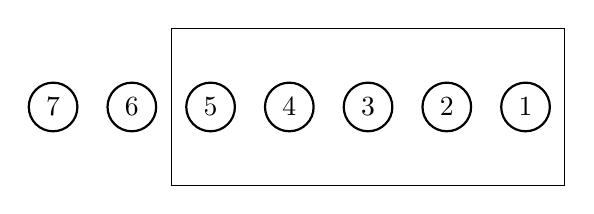
\begin{tikzpicture}
                \node[draw,circle,thick] at (1,1) {7};
                \node[draw,circle,thick] at (2,1) {6};
                \node[draw,circle,thick] at (3,1) {5};
                \node[draw,circle,thick] at (4,1) {4};
                \node[draw,circle,thick] at (5,1) {3};
                \node[draw,circle,thick] at (6,1) {2};
                \node[draw,circle,thick] at (7,1) {1};
                \draw (2.5,0) -- (7.5,0) -- (7.5,2) -- (2.5,2) -- (2.5,0);
            \end{tikzpicture}
          }
          \caption{理想情况}
      \end{figure}

      \begin{figure}
          \centering
          \scalebox{.8}{
            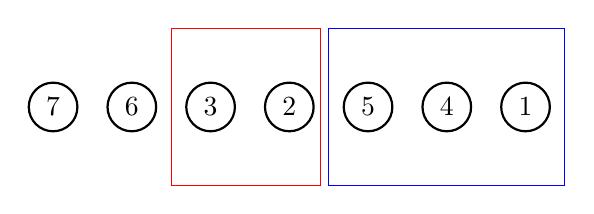
\begin{tikzpicture}
                \node[draw,circle,thick] at (1,1) {7};
                \node[draw,circle,thick] at (2,1) {6};
                \node[draw,circle,thick] at (3,1) {3};
                \node[draw,circle,thick] at (4,1) {2};
                \node[draw,circle,thick] at (5,1) {5};
                \node[draw,circle,thick] at (6,1) {4};
                \node[draw,circle,thick] at (7,1) {1};
                \draw[blue] (4.5,0) -- (7.5,0) -- (7.5,2) -- (4.5,2) -- (4.5,0);
                \draw[red] (2.5,0) -- (4.4,0) -- (4.4,2) -- (2.5,2) -- (2.5,0);
            \end{tikzpicture}
          }
          \caption{乱序情况}
      \end{figure}
  
  \end{frame}

  \begin{frame}
      \frametitle{乱序数据的影响}

      \begin{itemize}
        \item 当Flink以Event Time模式处理数据流时,它会根据数据里的时间戳来处理基于时间的算子
        \item 由于网络、分布式等原因,会导致乱序数据的产生
        \item 乱序数据会让窗口计算不准确
      \end{itemize}
  
  \end{frame}

  \begin{frame}
      \frametitle{水位线(Watermark)}
  
      \begin{itemize}
          \item 怎样避免乱序数据带来计算不正确?
          \item 遇到一个时间戳达到了窗口关闭时间,不应该立刻触发窗口计算,而是等待一段时间,等迟到的数据来了再关闭窗口
          \item 要等多长时间?碰到含有10000s时间戳的事件,敢闭合0s ~ 5s滚动窗口吗?
      \end{itemize}
  
  \end{frame}

  \begin{frame}
      \frametitle{水位线(Watermark)}
  
      \begin{itemize}
          \item Watermark 是一种衡量 Event Time 进展的机制(逻辑时钟),可以设定延迟触发
          \item Watermark 是用于处理乱序事件的,而正确的处理乱序事件,通常用 Watermark 机制结合 Window 来实现;
          \item 数据流中的 Watermark 用于表示 Timestamp 小于 Watermark 的数据,都已经到达了,因此,Window 的执行也是由 Watermark 触发的(水位线 >= 窗口结束时间)。
          \item Watermark 用来让程序自己平衡延迟和结果正确性。
      \end{itemize}
  
  \end{frame}

  \begin{frame}
      \frametitle{水位线}
      \begin{tcolorbox}
      	Flink认为时间戳小于等于水位线的事件都已到达
      \end{tcolorbox}
  \end{frame}

\begin{frame}
	\frametitle{水位线}
	\begin{tcolorbox}
		水位线是一种逻辑时钟
	\end{tcolorbox}
\end{frame}

\begin{frame}
	\frametitle{水位线}
	\begin{tcolorbox}
		水位线由程序员编程插入到数据流中
	\end{tcolorbox}
\end{frame}

\begin{frame}
	\frametitle{水位线}
	\begin{tcolorbox}
		水位线是一种特殊的事件
	\end{tcolorbox}
\end{frame}

\begin{frame}
	\frametitle{水位线}
	\begin{tcolorbox}
		在事件时间的世界里,水位线就是时间
	\end{tcolorbox}
\end{frame}

\begin{frame}
	\frametitle{水位线}
	\begin{tcolorbox}
		水位线 = 观察到的最大时间戳 - 最大延迟时间 - 1毫秒
	\end{tcolorbox}
\end{frame}

\begin{frame}
	\frametitle{窗口}
	\begin{tcolorbox}
		\begin{itemize}
			\item 左闭右开区间
			\item $\left[ 0s,5s \right] \text{不包含}  5s \text{,其实是} \left[ 0,4999ms \right]$
		\end{itemize}
	\end{tcolorbox}
	
\end{frame}

\begin{frame}
	\frametitle{水位线}
	\begin{tcolorbox}
		水位线超过窗口结束时间,窗口闭合,默认情况下,迟到元素被抛弃
	\end{tcolorbox}
\end{frame}

\begin{frame}
	\frametitle{水位线}
	\begin{tcolorbox}
		\begin{itemize}
			\item Flink会在流的最开始插入一个时间戳为负无穷大的水位线
			\item Flink会在流的最末尾插入一个时间戳为正无穷大的水位线
		\end{itemize}
	\end{tcolorbox}
\end{frame}

  \begin{frame}
      \frametitle{Watermark的特点}

      \begin{figure}
        \centering
        \includegraphics[width=0.6\textwidth]{image28.png}
        \caption{水位线的特点}
      \end{figure}
  
      \begin{itemize}
          \item Watermark 是一条特殊的数据记录,由程序员编程产生
          \item 水位线是流中的特殊事件,由程序员编程插入到数据流中
          \item Watermark必须单调递增,以确保任务的事件时间时钟在向前推进,而不是在后退,(Watermark就是当前数据流的逻辑时钟)
          \item Watermark 与数据的时间戳相关
      \end{itemize}
  
  \end{frame}

  \begin{frame}
      \frametitle{Watermark的传递}

      \begin{figure}
        \centering
        \includegraphics[width=0.6\textwidth]{image51.png}
        \caption{水位线的特点}
      \end{figure}
  
  \end{frame}

  \begin{frame}[fragile]
      \frametitle{Watermark的引入}

      \begin{itemize}
          \item Event Time 的使用一定要指定数据源中的时间戳(单位是ms)
      \end{itemize}

\begin{minted}[linenos,breaklines,fontsize=\tiny]{java}
.assignTimestampsAndWatermarks(
    WatermarkStrategy
        .<SensorReading>forBoundedOutOfOrderness(Duration.ofSeconds(5))
        .withTimestampAssigner(new SerializableTimestampAssigner<SensorReading>() {
            @Override
            public long extractTimestamp(SensorReading element, long recordTimestamp) {
                return element.timestamp;
            }
        })
)
\end{minted}
  
  \end{frame}

  \begin{frame}[fragile]
      \frametitle{Watermark的引入}

      \begin{itemize}
          \item 对于排好序的数据,不需要延迟触发,可以只指定时间戳就行了。
      \end{itemize}
  
\begin{minted}[linenos,breaklines,fontsize=\tiny]{java}
.assignTimestampsAndWatermarks(
    WatermarkStrategy.<SensorReading>forMonotonousTimestamps()
    .withTimestampAssigner(new SerializableTimestampAssigner<SensorReading>() {
        @Override
        public long extractTimestamp(SensorReading element, long l) {
            return element.timestamp;
        }
    })
);
\end{minted}
  
  \end{frame}

  \begin{frame}[fragile]
      \frametitle{自定义水位线}
  
\begin{minted}[linenos,breaklines,fontsize=\tiny]{java}
@Public
public interface WatermarkGenerator<T> {

    /**
     * 每来一个事件都会调用, 允许水位线产生器记忆和检查事件的时间戳。
     * 允许水位线产生器基于事件本身发射水位线。
     */
    void onEvent(T event, long eventTimestamp, WatermarkOutput output);

    /**
     * 周期性的调用(默认200ms调用一次), 可能会产生新的水位线,也可能不会。
     *
     * 调用周期通过ExecutionConfig#getAutoWatermarkInterval()方法来配置。
     */
    void onPeriodicEmit(WatermarkOutput output);
}
\end{minted}
  
  \end{frame}

  \begin{frame}[fragile]
      \frametitle{周期性产生水位线}
  
\begin{minted}[linenos,breaklines,fontsize=\tiny]{java}
public class BoundedOutOfOrdernessGenerator implements WatermarkGenerator<MyEvent> {

    private final long maxOutOfOrderness = 3500; // 最大延迟时间是3.5s

    private long currentMaxTimestamp;

    @Override
    public void onEvent(MyEvent event, long eventTimestamp, WatermarkOutput output) {
        currentMaxTimestamp = Math.max(currentMaxTimestamp, eventTimestamp);
    }

    @Override
    public void onPeriodicEmit(WatermarkOutput output) {
        // 产生水位线的公式:观察到的最大时间戳 - 最大延迟时间 - 1ms
        output.emitWatermark(new Watermark(currentMaxTimestamp - maxOutOfOrderness - 1));
    }

}
\end{minted}
  
  \end{frame}

  \begin{frame}[fragile]
      \frametitle{不规则水位线的产生}
  
\begin{minted}[linenos,breaklines,fontsize=\tiny]{java}
public class PunctuatedAssigner implements WatermarkGenerator<MyEvent> {

    @Override
    public void onEvent(MyEvent event, long eventTimestamp, WatermarkOutput output) {
        if (event.hasWatermarkMarker()) {
            output.emitWatermark(new Watermark(event.getWatermarkTimestamp()));
        }
    }

    @Override
    public void onPeriodicEmit(WatermarkOutput output) {
        // 不需要做任何事情,因为我们在onEvent方法中发射了水位线
    }
}
\end{minted}
  
  \end{frame}

  \begin{frame}
      \frametitle{Watermark的设定}

      \begin{itemize}
          \item 在Flink中,Watermark由应用程序开发人员生成,这通常需要对相应的领域有一定的了解
          \item 如果Watermark设置的延迟太久,收到结果的速度可能就会很慢,解决办法是在水位线到达之前输出一个近似结果
          \item 而如果Watermark到达得太早,则可能收到错误结果,不过Flink处理迟到数据的机制可以解决这个问题          
      \end{itemize}
  
  \end{frame}

  \begin{frame}[plain,c]
    %\frametitle{A first slide}
    
    \begin{center}
    \Huge Q \& A
    \end{center}
    
  \end{frame}

\end{document}